\documentclass[11pt]{article}

\usepackage[margin=1in]{geometry}
\usepackage{amsmath,amssymb,mathtools}
\usepackage{booktabs}
\usepackage{graphicx}
\usepackage{float}

\setlength{\parindent}{0pt}
\setlength{\parskip}{0.55em}
\renewcommand{\arraystretch}{1.15}

\newcommand{\Oh}{\mathcal{O}}
\newcommand{\eoc}{\mathrm{EOC}}
\newcommand{\norm}[1]{\left\lVert #1\right\rVert}

\title{Problem 4 Handout II\\CNLF Finite-Difference Scheme for Viscous Burgers' Equation}
\author{Rishabh Kumar}
\date{\today}

\begin{document}
\maketitle

\section{Conservative Form}

The viscous Burgers' equation is
\begin{equation}
    u_t+u u_x=\varepsilon u_{xx}.
    \label{eq:burgers}
\end{equation}
Since
\begin{equation}
    u u_x=\frac{1}{2}(u^2)_x,
\end{equation}
we use the conservative form
\begin{equation}
    u_t+\frac{1}{2}(u^2)_x=\varepsilon u_{xx}.
    \label{eq:conservative}
\end{equation}
This form is important because the nonlinear term is treated as the derivative of a
flux:
\begin{equation}
    f(u)=\frac{u^2}{2}.
\end{equation}
For nonlinear conservation laws, discretising the flux difference is usually more
robust than discretising $u u_x$ directly.

\section{Grid and Notation}

Let
\begin{equation}
    x_m=x_L+mh,
    \qquad
    t_n=nk,
    \qquad
    V_m^n\approx u(x_m,t_n).
\end{equation}
Define the second-difference operator
\begin{equation}
    \delta_x^2 V_m^n
    =
    V_{m+1}^n-2V_m^n+V_{m-1}^n.
\end{equation}
The CNLF method combines three choices:
\begin{itemize}
    \item leap-frog in time for $u_t$;
    \item an explicit centred conservative difference for $(u^2)_x/2$;
    \item Crank--Nicolson averaging for the diffusion term $\varepsilon u_{xx}$.
\end{itemize}

\section{Derivation of the CNLF Scheme}

Approximate the time derivative at $(x_m,t_n)$ by
\begin{equation}
    u_t(x_m,t_n)
    \approx
    \frac{V_m^{n+1}-V_m^{n-1}}{2k}.
\end{equation}
Approximate the conservative nonlinear flux by
\begin{equation}
    \frac12(u^2)_x(x_m,t_n)
    \approx
    \frac{1}{2}
    \frac{(V_{m+1}^n)^2-(V_{m-1}^n)^2}{2h}
    =
    \frac{(V_{m+1}^n)^2-(V_{m-1}^n)^2}{4h}.
\end{equation}
Finally, approximate diffusion by a Crank--Nicolson average over the two leap-frog
levels:
\begin{equation}
    u_{xx}(x_m,t_n)
    \approx
    \frac{1}{2}
    \left(
        \frac{\delta_x^2 V_m^{n+1}}{h^2}
        +
        \frac{\delta_x^2 V_m^{n-1}}{h^2}
    \right).
\end{equation}
Substituting these into \eqref{eq:conservative} gives
\begin{equation}
    \frac{V_m^{n+1}-V_m^{n-1}}{2k}
    +
    \frac{(V_{m+1}^n)^2-(V_{m-1}^n)^2}{4h}
    =
    \frac{\varepsilon}{2h^2}
    \left(
        \delta_x^2V_m^{n+1}
        +
        \delta_x^2V_m^{n-1}
    \right).
    \label{eq:raw-cnlf}
\end{equation}
Multiplying by $2k$ and setting
\begin{equation}
    \mu=\frac{\varepsilon k}{h^2},
\end{equation}
we obtain the practical update
\begin{equation}
    V_m^{n+1}-\mu\delta_x^2V_m^{n+1}
    =
    V_m^{n-1}+\mu\delta_x^2V_m^{n-1}
    -
    \frac{k}{2h}
    \left((V_{m+1}^n)^2-(V_{m-1}^n)^2\right).
    \label{eq:cnlf-update}
\end{equation}

\section{Linear System at Each Step}

Although Burgers' equation is nonlinear, the CNLF update is linear in the new unknowns
$V^{n+1}$.  The nonlinear flux is evaluated at time level $n$, so it is already known
when solving for $V^{n+1}$.

Expanding the left-hand side of \eqref{eq:cnlf-update},
\begin{equation}
    V_m^{n+1}
    -
    \mu
    \left(
        V_{m+1}^{n+1}
        -2V_m^{n+1}
        +V_{m-1}^{n+1}
    \right)
    =
    -\mu V_{m-1}^{n+1}
    +(1+2\mu)V_m^{n+1}
    -\mu V_{m+1}^{n+1}.
\end{equation}
Thus, for interior nodes, the new solution is obtained from a tridiagonal linear
system with coefficients
\begin{equation}
    \text{subdiagonal}=-\mu,
    \qquad
    \text{diagonal}=1+2\mu,
    \qquad
    \text{superdiagonal}=-\mu.
\end{equation}
Known boundary values at the new time are moved to the right-hand side.  This is why
the travelling-wave test can impose exact boundary values from the exact solution.

\section{Two-Step Startup}

CNLF is a two-step method.  To compute $V^{n+1}$, it needs both $V^n$ and $V^{n-1}$.
Therefore a computation must provide
\begin{equation}
    V^0\approx u(\cdot,0),
    \qquad
    V^1\approx u(\cdot,k).
\end{equation}
For the travelling-wave convergence tests, the notebook uses the exact travelling wave
to set $V^1$.  This isolates the accuracy of the CNLF update itself.  For a general
problem, one may instead compute $V^1$ with a one-step Crank--Nicolson startup.

\section{Error Norms and Observed Rates}

For a final time $T=t_N$, define the grid error
\begin{equation}
    e_m^N=V_m^N-u(x_m,T).
\end{equation}
The maximum norm and discrete $L^2$ norm used in the tables are
\begin{equation}
    \norm{e^N}_\infty=\max_m |e_m^N|,
    \qquad
    \norm{e^N}_2=
    \left(h\sum_m |e_m^N|^2\right)^{1/2}.
\end{equation}
For two successive errors $E_h$ and $E_{h/2}$, the observed rate is
\begin{equation}
    \eoc=
    \frac{\log(E_h/E_{h/2})}{\log 2}.
\end{equation}

\section{Local Truncation Error}

Let $u_m^n=u(x_m,t_n)$ be the exact smooth solution sampled on the grid, and let
\begin{equation}
    q(x,t)=u(x,t)^2.
\end{equation}
The leap-frog time difference satisfies
\begin{equation}
    \frac{u_m^{n+1}-u_m^{n-1}}{2k}
    =
    u_t+\frac{k^2}{6}u_{ttt}+\Oh(k^4).
    \label{eq:time-expansion}
\end{equation}
The conservative nonlinear flux satisfies
\begin{align}
    \frac{(u_{m+1}^n)^2-(u_{m-1}^n)^2}{4h}
    &=
    \frac{1}{2}
    \frac{q(x_m+h,t_n)-q(x_m-h,t_n)}{2h}
    \\
    &=
    \frac12 q_x+\frac{h^2}{12}q_{xxx}+\Oh(h^4)
    \\
    &=
    \frac12(u^2)_x+\frac{h^2}{12}(u^2)_{xxx}+\Oh(h^4).
    \label{eq:flux-expansion}
\end{align}
For the diffusion term,
\begin{equation}
    \frac{\delta_x^2u_m^{n\pm1}}{h^2}
    =
    u_{xx}(x_m,t_{n\pm1})
    +
    \frac{h^2}{12}u_{xxxx}(x_m,t_{n\pm1})
    +
    \Oh(h^4).
\end{equation}
Averaging the two time levels gives
\begin{align}
    \frac{\delta_x^2u_m^{n+1}+\delta_x^2u_m^{n-1}}{2h^2}
    &=
    u_{xx}
    +
    \frac{k^2}{2}u_{xxtt}
    +
    \frac{h^2}{12}u_{xxxx}
    +
    \Oh(k^4+k^2h^2+h^4).
    \label{eq:diffusion-expansion}
\end{align}
Substituting the exact solution into the discrete residual, and using
\eqref{eq:conservative}, gives
\begin{equation}
\begin{aligned}
    \tau_m^n
    &=
    \frac{k^2}{6}u_{ttt}
    +
    \frac{h^2}{12}(u^2)_{xxx}
    -
    \varepsilon
    \left(
        \frac{k^2}{2}u_{xxtt}
        +
        \frac{h^2}{12}u_{xxxx}
    \right)
    \\
    &\qquad
    +
    \Oh(k^4+k^2h^2+h^4).
\end{aligned}
\end{equation}
Therefore
\begin{equation}
    \boxed{\tau_m^n=\Oh(k^2+h^2).}
\end{equation}
This is a smooth-solution consistency statement.  With a second-order startup and a
stable computation, one expects second-order global convergence.

\section{Travelling-Wave Convergence Data}

The manufactured exact solution is the travelling wave with
\begin{equation}
    \omega=0.5,
    \qquad
    \varepsilon=0.1,
    \qquad
    x_0=3,
    \qquad
    -5\le x\le5,
    \qquad
    T=2.
\end{equation}
For the high-resolution run with $h=k=10^{-3}$, the notebook reports
\begin{equation}
    \norm{e(T)}_\infty=4.548\times10^{-7}.
\end{equation}

\begin{figure}[H]
    \centering
    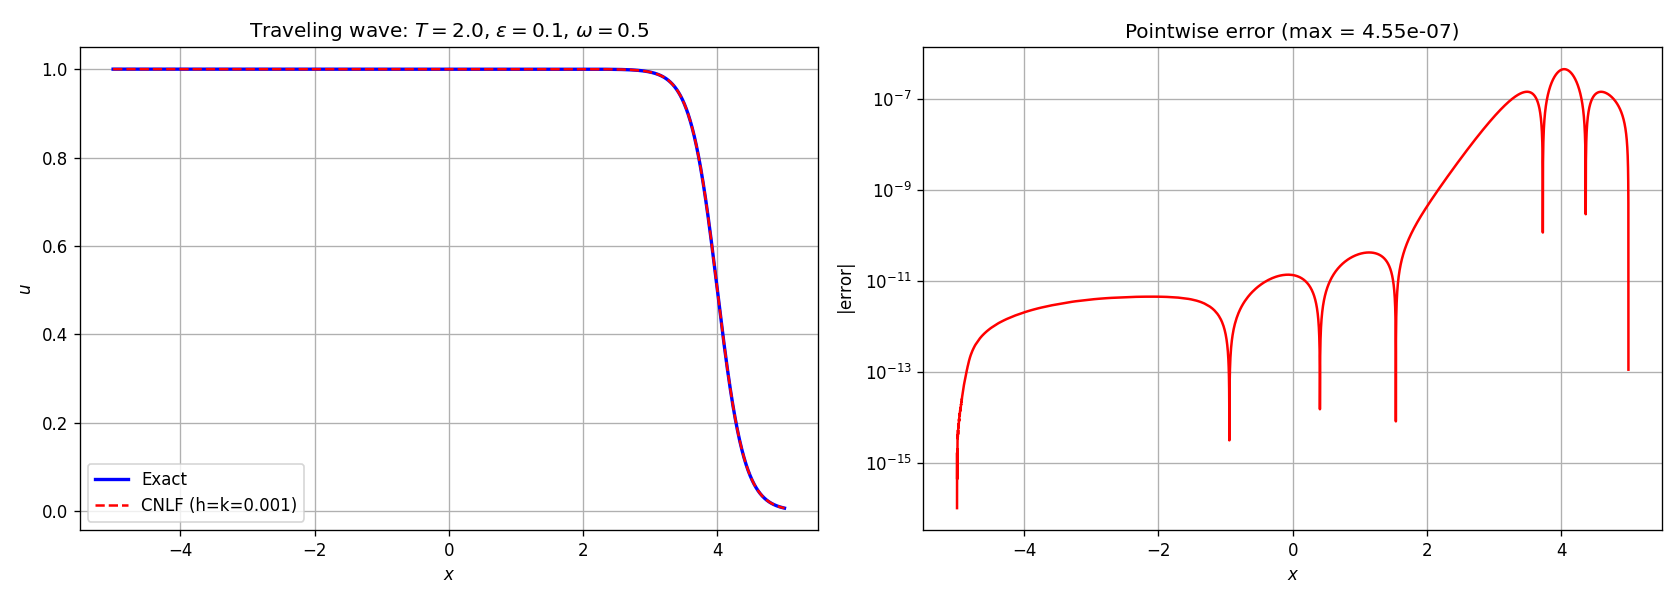
\includegraphics[width=\textwidth]{figures/traveling_wave.png}
    \caption{CNLF travelling-wave computation and pointwise absolute error.}
\end{figure}

\begin{table}[H]
    \centering
    \caption{Coupled convergence with $h=k$.}
    \begin{tabular}{@{}ccc@{}}
        \toprule
        $h=k$ & $\norm{e(T)}_\infty$ & rate \\
        \midrule
        0.0400 & $6.056\times10^{-4}$ & -- \\
        0.0200 & $1.513\times10^{-4}$ & 2.001 \\
        0.0100 & $3.790\times10^{-5}$ & 1.997 \\
        0.0050 & $9.485\times10^{-6}$ & 1.998 \\
        \bottomrule
    \end{tabular}
\end{table}

\begin{figure}[H]
    \centering
    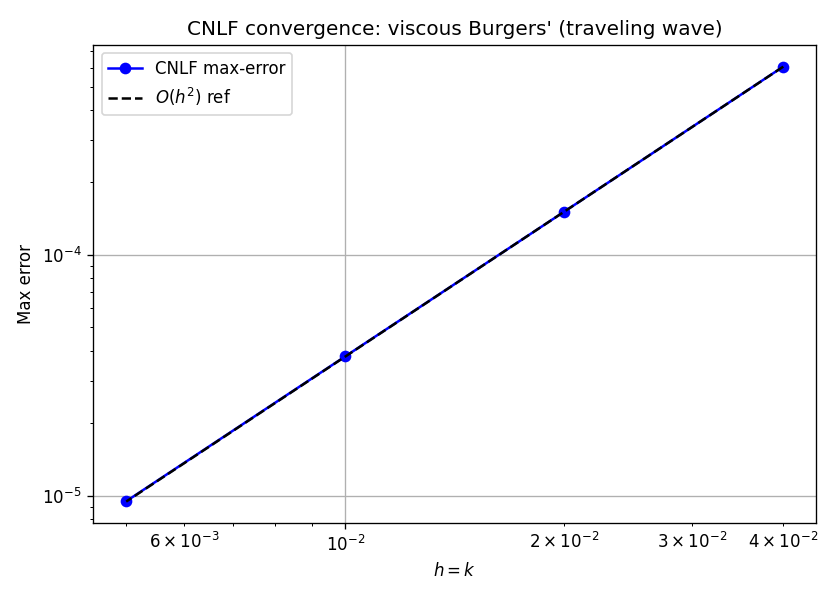
\includegraphics[width=0.72\textwidth]{figures/burgers_convergence.png}
    \caption{Coupled second-order convergence for the CNLF finite-difference method.}
\end{figure}

\section{Separate Time and Space Convergence}

To isolate time accuracy, the spatial mesh is made very fine:
\begin{equation}
    h=2.5\times10^{-4}.
\end{equation}
Then the measured $L^2$ error behaves as $O(k^2)$.

\begin{table}[H]
    \centering
    \caption{Temporal convergence with $h=2.5\times10^{-4}$.}
    \begin{tabular}{@{}ccc@{}}
        \toprule
        $k$ & $\norm{e}_2$ & rate \\
        \midrule
        $8.0\times10^{-3}$ & $3.663\times10^{-6}$ & -- \\
        $4.0\times10^{-3}$ & $9.125\times10^{-7}$ & 2.005 \\
        $2.0\times10^{-3}$ & $2.250\times10^{-7}$ & 2.020 \\
        $1.0\times10^{-3}$ & $5.316\times10^{-8}$ & 2.081 \\
        \bottomrule
    \end{tabular}
\end{table}

To isolate space accuracy, the time step is made very small:
\begin{equation}
    k=10^{-4}.
\end{equation}
Then the measured $L^2$ error behaves as $O(h^2)$.

\begin{table}[H]
    \centering
    \caption{Spatial convergence with $k=10^{-4}$.}
    \begin{tabular}{@{}ccc@{}}
        \toprule
        $h$ & $\norm{e}_2$ & rate \\
        \midrule
        $4.0\times10^{-2}$ & $1.584\times10^{-4}$ & -- \\
        $2.0\times10^{-2}$ & $3.963\times10^{-5}$ & 1.999 \\
        $1.0\times10^{-2}$ & $9.911\times10^{-6}$ & 1.999 \\
        $5.0\times10^{-3}$ & $2.478\times10^{-6}$ & 2.000 \\
        \bottomrule
    \end{tabular}
\end{table}

\begin{figure}[H]
    \centering
    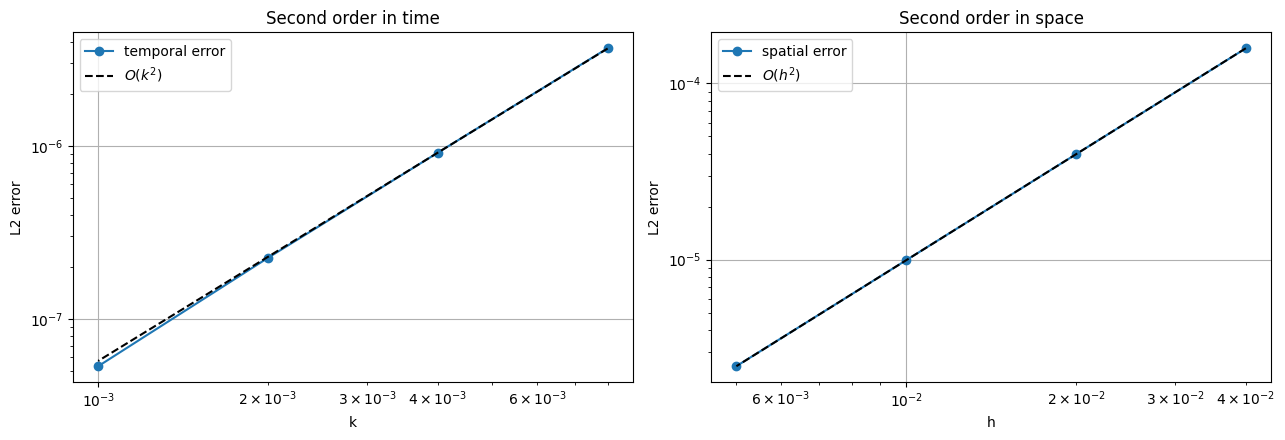
\includegraphics[width=0.9\textwidth]{figures/individual_second_order.png}
    \caption{Separate temporal and spatial convergence tests.}
\end{figure}

\section{Conclusion}

The finite-difference method is second order because each of its three components is
second order in the appropriate sense: leap-frog is second order in time, the centred
flux difference is second order in space, and the diffusion term uses a
Crank--Nicolson average with a centred second difference.  The convergence tables
confirm the expected $\Oh(k^2+h^2)$ behaviour.

\end{document}
